% !TeX spellcheck = cs_CZ
%%%%%%%%%%%%%%%%%%%%%%%%%%%%%%%%%%%%%%%%%
% University Assignment Title Page 
% LaTeX Template
% Version 1.0 (27/12/12)
%
% This template has been downloaded from:
% http://www.LaTeXTemplates.com
%
% Original author:
% WikiBooks (http://en.wikibooks.org/wiki/LaTeX/Title_Creation)
%
% License:
% CC BY-NC-SA 3.0 (http://creativecommons.org/licenses/by-nc-sa/3.0/)
% 
% Instructions for using this template:
% This title page is capable of being compiled as is. This is not useful for 
% including it in another document. To do this, you have two options: 
%
% 1) Copy/paste everything between \begin{document} and \end{document} 
% starting at \begin{titlepage} and paste this into another LaTeX file where you 
% want your title page.
% OR
% 2) Remove everything outside the \begin{titlepage} and \end{titlepage} and 
% move this file to the same directory as the LaTeX file you wish to add it to. 
% Then add \input{./title_page_1.tex} to your LaTeX file where you want your
% title page.
%
%%%%%%%%%%%%%%%%%%%%%%%%%%%%%%%%%%%%%%%%%

%----------------------------------------------------------------------------------------
%	PACKAGES AND OTHER DOCUMENT CONFIGURATIONS
\documentclass[czech,12pt]{article}
\usepackage[T1]{fontenc}
\usepackage[utf8]{inputenc}
\usepackage[czech]{babel}
\usepackage{graphicx}
\usepackage{hyperref}
\usepackage{listings}
%----------------------------------------------------------------------------------------

\hyphenation{OpenMP}

\begin{document}

\begin{titlepage}
\newcommand{\HRule}{\rule{\linewidth}{0.5mm}} % Defines a new command for the horizontal lines, change thickness here
\center

\textsc{\LARGE Fakulta informačních technologií}\\[1.5cm] % Jmeno fakulty (university)
\textsc{\Large Paralelní architektury počítačů}\\[0.5cm] % Nazev predmetu
\textsc{\large technická zpráva}\\[0.5cm] % Druh zpravy


% TITLE
\HRule \\[0.4cm]
{ \huge \bfseries Hledání nejkratších cest v~grafu}\\[0.4cm] % Nazev dokumentu (prace)
\HRule \\[1.5cm]

% AUTOR
\Large \emph{Autoři:}\\
Vojtěch \textsc{Myslivec}\\
Zdeněk \textsc{Nový}\\[2cm]	% Jmeno

% DATUM
{\large \today}\\[3cm] % Datum zmeny jako dnesek

% LOGO

\includegraphics{cvut-logo-bw.pdf}\\[1cm] % Vlozene logo (nutny balik graphicx)

\vfill % Zbytek stranky neni nic
\end{titlepage}

%--- Abstrakt ---
\renewcommand\abstractname{\begin{flushright}\begin{LARGE}\textbf{Abstrakt}\end
{LARGE}\end{flushright}}
\newcommand{\keywords}[1]{\vspace{0.8cm}\textbf{Klíčová slova\hspace{0.2cm}} #1}
\noindent\makebox[\linewidth]{\rule{\textwidth}{0.4pt}}
\begin{abstract}
Účelem této práce je sumarizovat výsledky měření řešení problému hledání nejkratších cest v~grafu (NCG). Práce se zaměřuje na řešení problému Dijkstrovým a~Floyd-Warshallovým algoritmem a~porovnání sekvenční a~několika paralelních implementací.
\end{abstract}

% --- Klicova slova ---
\keywords{Dijkstra, Floyd-Warshall, nejkratší cesty, NCG, OpenMP, Cuda}

\clearpage

%-------------------------------
%---		   Obsah	 	 ---
%-------------------------------
\tableofcontents

\clearpage

%-------------------------------
%---		   Uvod		 	 ---
%-------------------------------
\section{Úvod}
Tato práce se zabývá implementací dvou algoritmů hledání nejkratších cest v~grafu. Jedná se o~implementaci sekvenčním algoritmem, který je poté paralelizován pro procesor a~pro grafickou kartu. Pro jednotlivé algoritmy je provedeno měření, které si klade za cíl určit zrychlení paralelních algoritmů proti sekvenčnímu.

%-------------------------------
%---			NCG			 ---
%-------------------------------
\section{Hledání nejkratších cest v~grafu} \label{ncg}
\subsection{Definice} \label{l:clondike:ncgdef}
Hledání nejkratších cest v~grafu je NP-úplná grafová úloha, jejímž cílem je nalézt v~zadaném grafu nejkratší cesty mezi všemi možnými dvojicemi uzlů A~a~B \cite{w:ncg}.

\subsection{Algoritmy}
\subsubsection{Dijkstrův algoritmus}
Dijkstrův algoritmus slouží k~nalezení všech nejkratších cest ze zadaného uzlu do všech ostatních uzlů grafu. Graf nesmí obsahovat hrany se zápornou délkou \cite{w:dij:def}.

\paragraph{Princip}
Dijkstrův algoritmus je zobecněné prohledávání grafu do šířky, při kterém se vlna šíří na základě vzdálenosti od zdrojového uzlu. K~uchovávání uzlů slouží prioritní fronta, která je řazena podle vzrůstající vzdálenosti od zdroje. V~každém kroku algoritmu je vybrán uzel s~nejmenší vzdáleností a~pro každého souseda je vypočítána jeho vzdálenost od zdrojového uzlu \cite{w:dij:def}.

\subsubsection{Floyd-Warshallův algoritmus}
Floyd-Warshallův algoritmus slouží k~nalezení nejkratších cest mezi všemi dvojicemi uzlů v~grafu. Graf může obsahovat hrany -- nikoliv však cykly -- se zápornou hodnotou délky\footnote{Pokud má graf cyklus se zápornou hodnotou délky, postrádá úloha nejkratších cest smysl.}~\cite{w:fw:def}.

\paragraph{Princip} \label{l:fw:princip}
Floyd-Warhsallův algoritmus pracuje s~maticí sousednosti, kde hrana je ohodnocena vahou. Na počátku tato matice obsahuje pouze vzdálenosti dvou uzlů, mezi kterými je vedena hrana. V~každém kroku je vybrán jeden uzel jako prostředník. Prvek matice sousednosti se přepočítá, pokud je vzdálenost z~počátečního do koncového uzlu kratší přes nového prostředníka než bez něj \cite{w:fw:def}.


%-------------------------------
%---		Sekvencni		 ---
%-------------------------------
\section{Sekvenční algoritmus}
\subsection{Společná implementace}
Oba algoritmy vycházejí z~obecněho principu, který je popsán v~kapitole \ref{l:fw:princip}. Algoritmy pracují s~grafem, který je programu předložen jako soubor, ve kterém je graf ve formě matice sousednosti. Společnou částí je tedy načítání vstupu a~jeho kontrola.

\subsection{Dijkstrův algoritmus}
Protože Dijkstrův algoritmus slouží k~hledání nejkratších cest od jednoho zdrojového uzlu, je nutné jej spouštět pro každý uzel grafu. To zajišťuje funkce \textit{dijkstraNtoN}.

\subsubsection{Dijkstrův algoritmus z~jednoho zdroje}
Pro výpočet Dijkstrova algoritmu z~jednoho zdrojového uzlu se alokují tři pole o~velikosti počtu uzlů. V~jednom je uložena vzdálenost daného uzlu od zdrojového, ve druhém předchozí uzel v~nalezené nejkratší cestě. Třetí pole určuje, jestli je už uzel uzavřený pro výpočty.

Algoritmus prochází postupně, podle nejmenší vzdálenosti, všechny uzly, které se nacházejí v~prioritní frontě. Z~daného uzlu vypočítá pro každého svého souseda novou cestu, která by vedla přes uzel samotný a~porovná ji s~dosavadní vzdáleností souseda. Menší vzdálenost je zapsána do pole vzdáleností a~algoritmus pokračuje.

\paragraph{Prioritní fronta} \label{l:dij:fron}
Za účelem prioritní fronty byla implementována binární halda, kde složitost výběru minima je logaritmická, oproti nativní implementaci pomocí pole, kde je složitost výběru minima lineární.


\subsubsection{Vektorizace}
Pomocí přepínačů optimalizace \textit{-O3} a~podpory vektorových sad \textit{-msse4.2} kompilátoru \textit{gcc} byla zapnuta podpora vektorizace cyklů \cite{w:vect}. Pro záznam o~pokusech vektorizace byl použit přepínač \textit{-ftree-vectorizer-verbose=n}, kde za \textit{n} byly dosazeny 1,~3,~5, kde čím vyšší číslo, tím podrobnější informace \cite{w:vect}.\textbf{}

Samotný algoritmus je velmi sekvenční. V každém kroku se vybere minimum z prioritní fronty --- jinými slovy ze složitější struktury --- a přepíší se hodnoty uzlu ve frontě. Tyto operace nelze nijak vektorizovat a~v~průběhu výpočtu (kromě počáteční inicializace polí) se nevyskytují žádné prvky vedle sebe ani pro čtení ani pro zápis.

% ----------------------------------------------------
% - vektorizovany cyklus -
\begin{figure}
    \centering
	\caption{Úspěšně vektorizovaný cyklus.}
	\label{f:dij:vect1}
    \begin{lstlisting}
dijkstra.cpp:38: note: LOOP VECTORIZED.
dijkstra.cpp:28: note: vectorized 1 loops in function.
    \end{lstlisting}
	\begin{lstlisting}
for ( unsigned j = 0; j < pocetUzlu; j++ ) {
	vzdalenostM[i][j] = DIJKSTRA_NEKONECNO;
	predchudceM[i][j] = DIJKSTRA_NEDEFINOVANO;
}
    \end{lstlisting}
    
    \begin{lstlisting}
dijkstra.cpp:99: note: not vectorized: number of iterations cannot be computed.
dijkstra.cpp:99: note: bad loop form.
dijkstra.cpp:82: note: vectorized 0 loops in function.
    \end{lstlisting}
\end{figure}
% ----------------------------------------------------
% - nevektorizovany cyklus -
\begin{figure}
    \centering
    \caption{Cyklus, který se nepodařilo vektorizovat.}
	\label{f:dij:vect2}
    \begin{lstlisting}
dijkstra.cpp:99: note: not vectorized: number of iterations cannot be computed.
dijkstra.cpp:99: note: bad loop form.
dijkstra.cpp:82: note: vectorized 0 loops in function.
    \end{lstlisting}
    
	\begin{lstlisting}
for ( unsigned i = 0 ; i < pocetUzlu ; i++ ) {
	vzdalenostM[idUzlu][i] = vzdalenost[i];
	predchudceM[idUzlu][i] = predchudce[i];
}
	\end{lstlisting}
\end{figure}
% ----------------------------------------------------

\paragraph{Původní stav}
Na obrázcích \ref{f:dij:vect1} a~\ref{f:dij:vect2} je znázorněn příklad jednoho z cyklů, který byl vektorizován a~jiný cyklus, který se nepodařilo vektorizovat z~důvodu neznámého počtu iterací.

\paragraph{Optimalizace}
Výpis \ref{f:dij:vect3} ukazuje úspěšnou úpravu cyklu, který se díky změně zdrojového kódu podařilo vektorizovat.

% ----------------------------------------------------
% - upraveny vektorizovany cyklus -
\begin{figure}
    \centering
    \caption{Upravený cyklus, aby mohl být vektorizován.}
	\label{f:dij:vect3}
    \begin{lstlisting}
Vectorizing loop at dijkstra.cpp:99
dijkstra.cpp:99: note: LOOP VECTORIZED.
dijkstra.cpp:82: note: vectorized 1 loops in function.
    \end{lstlisting}
    
	\begin{lstlisting}
unsigned tmp = pocetUzlu;
for ( unsigned i = 0 ; i < tmp ; i++ ) {
	vzdalenostM[idUzlu][i] = vzdalenost[i];
	predchudceM[idUzlu][i] = predchudce[i];
}
	\end{lstlisting}
\end{figure}
% ----------------------------------------------------

% \paragraph{Optimalizace}
% Výpis \ref{f:dij:vect3} dokazuje úspěšnou úpravu cyklu, který se, díky malé změně zdrojového kódu, podařilo vektorizovat.

%\subsubsection{Optimalizace}


\subsection{Floyd-Warshallův algoritmus}
Floyd-Warshallův algoritmus obsahuje tři vnořené for cykly a~funguje na principu popsaném v~\ref{l:fw:princip}. Jako datové struktury používá čtyři matice o~velikosti počtu uzlů $\times$ počet uzlů. Pro každý uzel si algoritmus udržuje aktuální vzdálenosti ke všem uzlům a~navíc vzdálenosti z~předchozí iterace. Další dvě matice obsahují předchozí uzel v~nalezené cestě. 

\subsection{Implementace}
Aktuální implementace je k~nahlédnutí i~ke stažení na adrese \url{https://github.com/VojtechMyslivec/PAP-NCG}. Sekvenční algoritmus se nachází ve složce \textit{01\_sekvencni}.

\subsubsection{Vektorizace}
Algoritmus sice počítá s maticemi, ale během výpočtu se porovnávají čísla, která v dané matici nemusí vůbec sousedit (navíc se porovnávají pouze dvě čísla: jedno na indexu \emph{(i,j)} a druhé, které je součtem dvou čísel na indexech \emph{(i,k)} a \emph{(k,j)}).
Z~výpisu \ref{f:fw:vect1} je patrné, že v~programu je vektorizován pouze cyklus pro inicializaci matic. 

% - vektorizovany cyklus -
\begin{figure}
    \centering
    \caption{Úspěšně vektorizovaný cyklus.}
	\label{f:fw:vect1}
    \begin{lstlisting}
floydWarshall.cpp:90: note: vectorizing stmts using SLP.BASIC BLOCK VECTORIZED
floydWarshall.cpp:90: note: basic block vectorized using SLP
    \end{lstlisting}
    
	\begin{lstlisting}
for ( unsigned k = 0; k < tmp; k++ ) {
	unsigned i;
	#pragma omp parallel for private( i, novaVzdalenost ) shared( delkaPredchozi, delkaAktualni, pre    dchudcePredchozi, predchudceAktualni )
	for ( i = 0; i < tmp; i++ ) {
		for ( unsigned j = 0; j < tmp; j++ ) {
	\end{lstlisting}
\end{figure}


%\subsubsection{Optimalizace}


%-------------------------------
%---		OpenMP			 ---
%-------------------------------
\section{Paralelní algoritmus pomocí knihovny OpenMP}

% ########## Dijkstra ##########
\subsection{Dijkstrův algoritmus} \label{l:omp:dij}
Paralelizace algoritmu spočívá v~paralelizaci cyklu, který prochází jednotlivé uzly a~pro ně řeší problém hledání nejkratší cesty v~grafu z~jednoho počátečního uzlu. Každé vlákno tedy zpracovává jeden uzel jako počáteční a~z~něj hledá nejkratší cesty do všech ostatních uzlů.

\subsubsection{Paměťové struktury}
Každé vlákno dostane ukazatel na strukturu grafu. Protože všechna vlákna používají strukturu grafu pouze ke čtení, nedochází při přístupu k~této struktuře k~žádným datovým hazardům.

Každé vlákno si vytvoří jeden objekt, ve kterém si alokuje vlastní pole vzdáleností a~předchůdců, které používá pro své výpočty. Tyto struktury jsou po ukončení funkce vlákna dealokovány společně s~objektem.

\subsubsection{Úprava algoritmu}
Z~důvodu paralelizace algoritmu bylo nutné upravit použitou prioritní frontu. V~sekvenčním řešení byla použita implementace pomocí binární haldy \ref{l:dij:fron}. Z~důvodu paralelizace výběru minima z~fronty je pro paralelní řešení výhodnější použít implementaci polem.


% ########## Floyd - Warshall ##########
\subsection{Floyd-Warshallův algoritmus}
Díky třem vnořeným sekvenčního algoritmu existuje několik možností, jak algoritmus paralelizovat.

\subsubsection{První varianta}
První variantou je algoritmus paralelizovat pouze v~jednom cyklu, který definuje, která řádka je právě zpracovávána. 
Vlákna čtou z~matice $W_k$ a~zapisují do přidělených řádků v~matici $W_{k+1}$\footnote{V každém kroku je
potřeba pouze jedna matice z předchozí iterace a~jedna matice pro zápis nalezených cest. Na konci každé iterace 
se pak prohodí matice aktuální s maticí předchozí a~mohou se tak nepotřebná starší data přepisovat.}. Přidělené řádky 
jsou navzájem disjunktní, takže nehrozí konflikt zápisů jednotlivými vlákny (viz obrázek \ref{f:fw:omp}).

% Přidělená data jednomu vláknu zobrazuje obrázek \ref{f:fw:omp}. Algoritmus zapisuje pouze do přidělených sloupců, tedy řádků zobrazených v~části \textit{a}. Řádek \textit{k} v~části \textit{b} využívají všechna vlákna pouze ke čtení, proto zde nedochází ke konfliktům. Tato varianta je implementována.

\begin{figure}
    \centering
    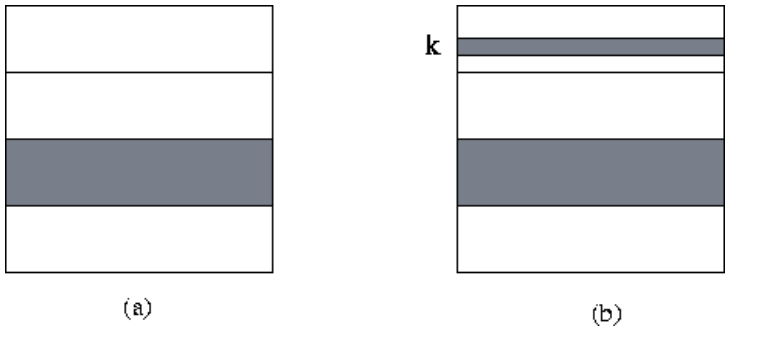
\includegraphics[width=\textwidth]{floyd-openmp}
    \caption{Ukázka dat přidělených jednomu vláknu při paralelizaci jednoho cyklu \cite{w:fw:omp}.}
    \label{f:fw:omp}
\end{figure}


\subsubsection{Druhá varianta}
Druhou variantou, jak problém paralelizovat je použít původní variantu a~přidat paralelizaci zároveň ve vnitřním cyklu, který prochází jednotlivé sloupce matice. V~takovém případě by jednomu vláknu byl přidělen jeden nebo více necelých řádků ohraničených sloupci. Tato varianta se jeví vhodnější pouze při velkém počtu dostupných vláken, proto není v~naší implementaci použita.

\subsection{Optimalizace implementace}
\subsubsection{Optimalizace vytváření vláken} \label{l:opt1}
Z měření algoritmu Floyd-Warshall v sekci \ref{l:vysledky} bylo zjištěno, že implementace v každé iteraci vnějšího cyklu vytváří a spouští nová vlákna, která po skončení vnitřního cyklu ukončí a v další iteraci proces opakuje. Proto byla paralelizace vláken upravena tak, aby na začátku vnějšího cyklu algoritmus vytvořil příslušný počet vláken, kterým pak v jednotlivých iteracích přiděloval práci. Grafy s touto optimalizací mají tvar \textit{*\_v2.png}. Výsledky měření jsou prezentovány v kapitole \ref{l:mer:opt1}.

\subsubsection{Odstranění výpočtu předchůdců} \label{l:opt2}
Protože zadáním této práce nebylo získat matici předchůdců, je v algoritmu zbytečné udržovat informaci o předchůdcích jednotlivých uzlů. Proto byly v rámci další optimalizace odstraněny veškeré výpočty, které se týkaly matice předchůdců. Výsledek byl znovu naměřen a výsledky jsou prezentovány v kapitolách \ref{l:mer:opt2}.


\subsection{Měření}
Na obou algoritmech bylo provedeno měření, které si klade za cíl analyzovat čas, zrychlení a~efektivitu použitého paralelního algoritmu. Měření bylo prováděno na hustých grafech, kde při generování grafů byla použita pravděpodobnost 0.5, že mezi dvěmi uzly existuje hrana.

\subsubsection{Testovací data}
Byly vygenerovány 2 testovací sady dat. Obě sady obsahují 25 grafů, kde pro každé $n$ (počet uzlů) z $1000$, $2000$, $3000$, $4000$ a $5000$ 
je vygenerováno 5 náhodných grafů. Jedna sada obsahuje \emph{husté} grafy s~pravděpodobností hrany $50 \%$, druhá obsahuje \emph{řídké} grafy
s~pravděpodobností hrany $1 \%$.
Měření probíhalo na serveru \url{star2.fit.cvut.cz} na stroji \textit{gpu-02} pro počet vláken $p$ $1$, $2$, $4$, $6$, $8$, $12$ a $24$.

Jako čas výpočtu pro dané $n$ se vypočítal průměr z časů přes všech 5 grafů s odpovídajícím počtem uzlů.

\subsubsection{Výsledky}
\label{l:vysledky}
Grafy \ref{f:mer:cas}, \ref{f:mer:zry} a~\ref{f:mer:efe} ukazují výsledky měření z~pohledu času, zrychlení a~efektivity.

% Cas
\begin{figure}
    \centering
    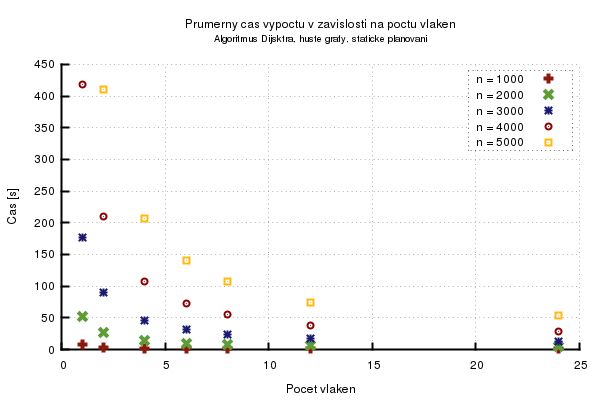
\includegraphics[width=0.45\textwidth]{../grafy/02_openMP/02-01-Dijkstra_cas_v1}
    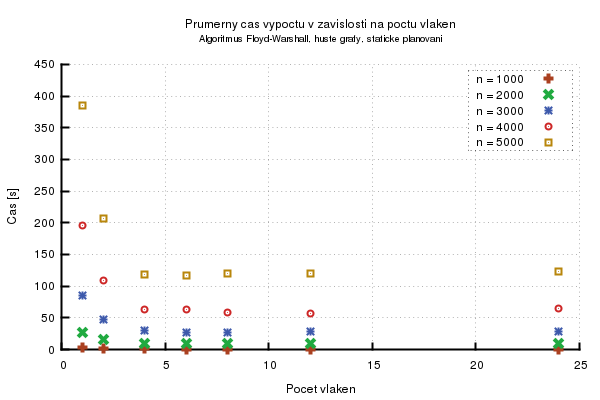
\includegraphics[width=0.45\textwidth]{../grafy/02_openMP/02-01-Floyd_cas_v1}
    \caption{Závislost průměrného času výpočtu v~závislosti na počtu vláken za použití statického plánování.}
    \label{f:mer:cas}
\end{figure}

% Zrychleni
\begin{figure}
    \centering
    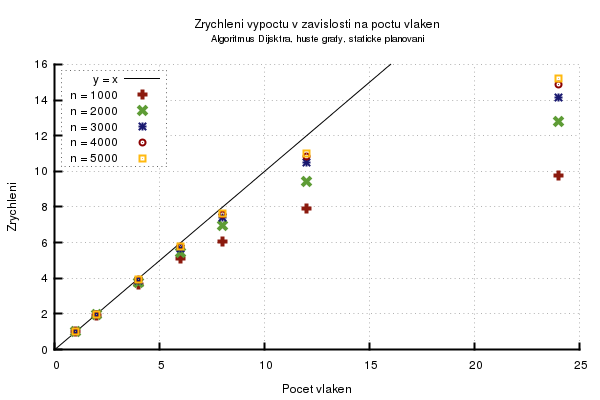
\includegraphics[width=0.45\textwidth]{../grafy/02_openMP/02-02-Dijkstra_zrychleni_v1}
    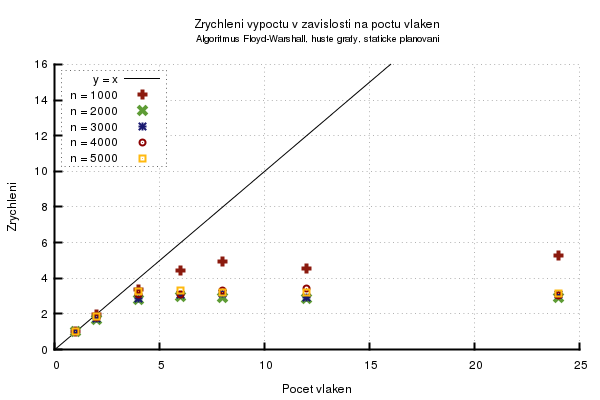
\includegraphics[width=0.45\textwidth]{../grafy/02_openMP/02-02-Floyd_zrychleni_v1}
    \caption{Závislost zrychlení paralelního algoritmu oproti sekvenčnímu v~závislosti na počtu vláken za použití statického plánování.}
    \label{f:mer:zry}
\end{figure}

% Efektivita
\begin{figure}
    \centering
    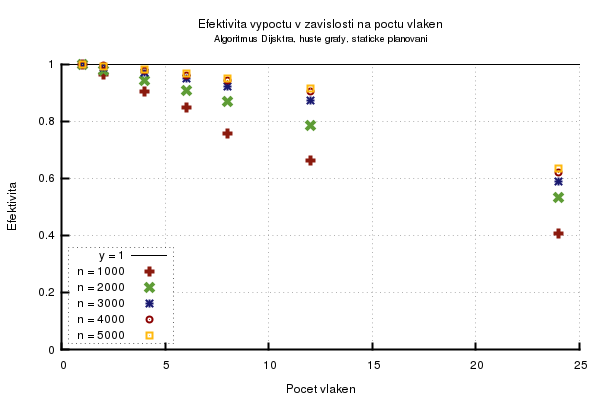
\includegraphics[width=0.45\textwidth]{../grafy/02_openMP/02-03-Dijkstra_efektivita_v1}
    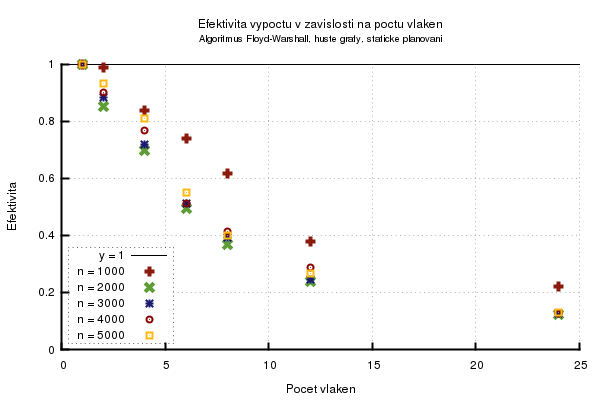
\includegraphics[width=0.45\textwidth]{../grafy/02_openMP/02-03-Floyd_efektivita_v1}
    \caption{Závislost efektivity algoritmu v~závislosti na počtu vláken za použití statického plánování.}
    \label{f:mer:efe}
\end{figure}

\paragraph{Poměr rychlosti algoritmů v závislosti na hustotě grafu}
Graf \ref{f:mer:pomerhustota} porovnává výpočetní časy při použití statického plánování v závislosti na hustotě grafu. Z grafů vyplývá, že oba algoritmy jsou téměř nezávislé na hustotě grafu.

\paragraph{Poměr rychlosti algoritmů v závislosti na plánování}
Graf \ref{f:mer:pomerplanovani} zobrazuje poměr výpočetních časů v závislosti na použitém plánování. V porovnání byla použita plánování statické a dynamické. Z grafů je patrné, že plánování ovlivní čas výpočtu pouze nevýznamně a není tedy podstatné, jaké plánování je v algoritmu použito.
\paragraph{Statické plánování}
Při statickém plánování se iterace cyklu rovnoměrně rozdělí po blocích mezi všechna vlákna před začátkem provádění cyklu \cite{w:omp}.
\paragraph{Dynamické plánování}
Dynamickým plánováním se rozumí rozdělení jednotlivých iterací vláknům po jedné iteraci. Vždy když vlákno dokončí iteraci, je mu přidělena další iterace \cite{w:omp}.

% Pomer rychlost vypoctu v zavislosti na hustote grafu
\begin{figure}
    \centering
    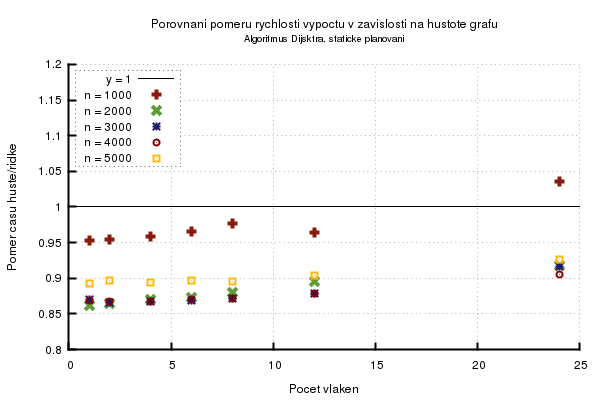
\includegraphics[width=0.45\textwidth]{../grafy/02_openMP/02-04-Dijkstra_hustota_v1}
    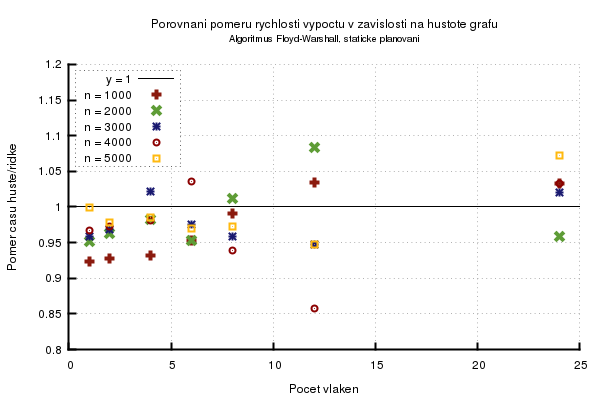
\includegraphics[width=0.45\textwidth]{../grafy/02_openMP/02-04-Floyd_hustota_v1}
    \caption{Porovnání poměru rychlostí výpočtu v závislosti na hustotě grafu při použití statického plánování.}
    \label{f:mer:pomerhustota}
\end{figure}

% Pomer rychlost vypoctu v zavislosti na hustote grafu
\begin{figure}
    \centering
    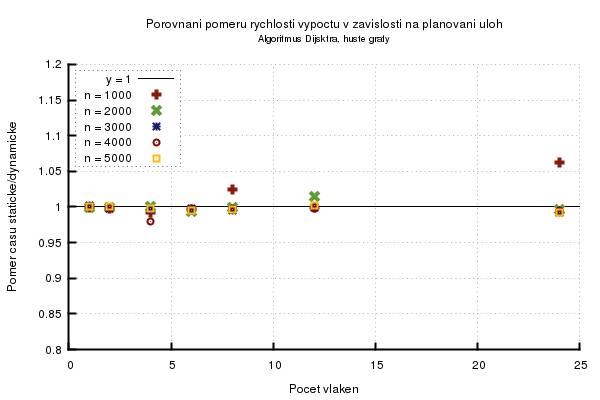
\includegraphics[width=0.45\textwidth]{../grafy/02_openMP/02-05-Dijkstra_schedule_v1}
    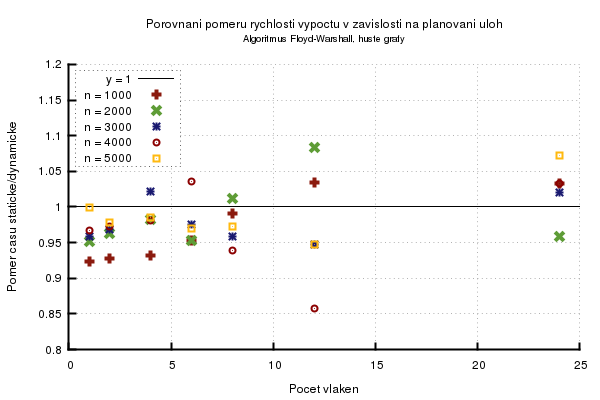
\includegraphics[width=0.45\textwidth]{../grafy/02_openMP/02-05-Floyd_schedule_v1}
    \caption{Porovnání poměru rychlostí výpočtu v závislosti na použitém plánování.}
    \label{f:mer:pomerplanovani}
\end{figure}

\subsubsection{Analýza}
\paragraph{Dijkstra}
Z~grafů \ref{f:mer:cas} je vidět klesající dobu výpočtu v závislosti na počtu vláken.
Zrychlení, které je zobrazeno v~grafu \ref{f:mer:zry} na počátku stoupá téměř lineárně a~teprve pro větší počet vláken 
se zmírňuje. Toto nelineární zrychlení může způsobit například přístup do paměti, protože se vzrůstajícím počtem vláken klesá 
relativní velikost cache pro každé z vláken.
Z~výše uvedeného vyplývá efektivita, která je zobrazena v~grafu \ref{f:mer:efe}.

\paragraph{Floyd-Warshallův algoritmus}
U~Floyd-Warshallova algoritmu se výpočetní čas pro počty vláken větší než 3 téměř nezkracuje. 
Zrychlení je tedy patrné pouze při použití 2 případně 4 vláknech. Z~výše uvedené plyne, že efektivita paralelního algoritmu velmi rychle klesá.

\subsubsection{Optimalizace vláken Floyd-Warshallova algoritmu} \label{l:mer:opt1}
Výsledky měření po implementaci optimalizace \ref{l:opt1} Floyd-Warshallova algoritmu.

% Cas po optimalizaci 
\begin{figure}
    \centering
    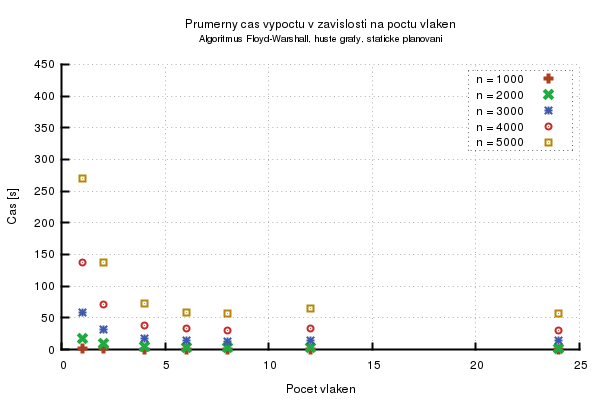
\includegraphics[width=0.45\textwidth]{../grafy/02_openMP/02-01-Floyd_cas_v2}
    \caption{Závislost průměrného času výpočtu v~závislosti na počtu vláken za použití statického plánování po optimalizaci \ref{l:opt1}.}
    \label{f:mer:cas:opt1}
\end{figure}

% Zrychleni
\begin{figure}
    \centering
    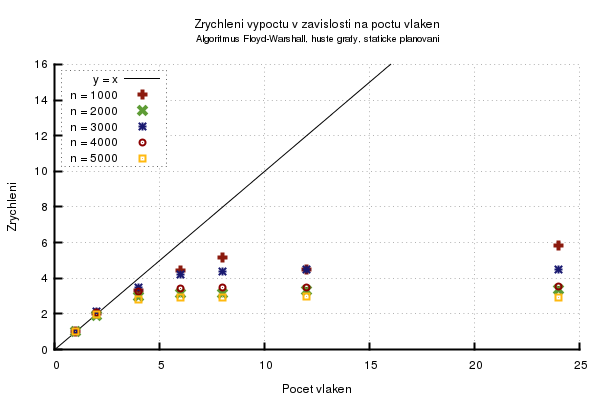
\includegraphics[width=0.45\textwidth]{../grafy/02_openMP/02-02-Floyd_zrychleni_v2}
    \caption{Závislost zrychlení paralelního algoritmu oproti sekvenčnímu v~závislosti na počtu vláken za použití statického plánovánípo optimalizaci \ref{l:opt1}.}
    \label{f:mer:zry:opt1}
\end{figure}

% Efektivita
\begin{figure}
    \centering
    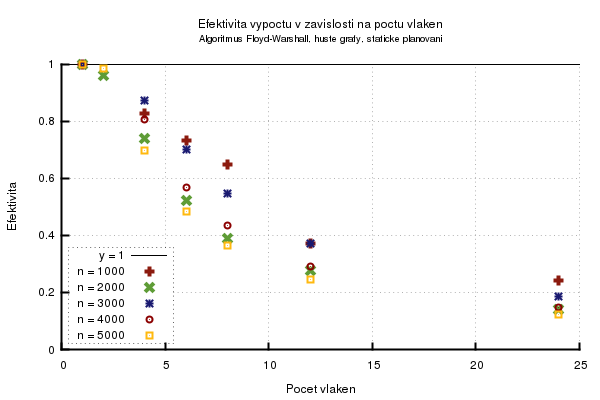
\includegraphics[width=0.45\textwidth]{../grafy/02_openMP/02-03-Floyd_efektivita_v2}
    \caption{Závislost efektivity algoritmu v~závislosti na počtu vláken za použití statického plánování po optimalizaci \ref{l:opt1}.}
    \label{f:mer:efe:opt1}
\end{figure}

\subsubsection{Optimalizace odstraněním předchůdců obou algoritmů} \label{l:mer:opt2}
Výsledky měření obou algoritmů po implementaci optimalizace \ref{l:opt2}.

% Cas po optimalizaci
\begin{figure}
    \centering
    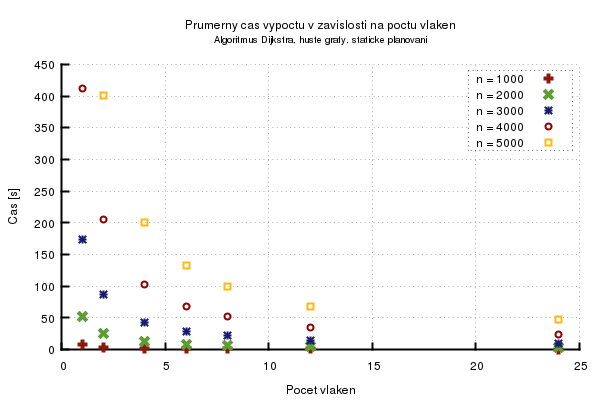
\includegraphics[width=0.45\textwidth]{../grafy/02_openMP/02-01-Dijkstra_cas_v3}
    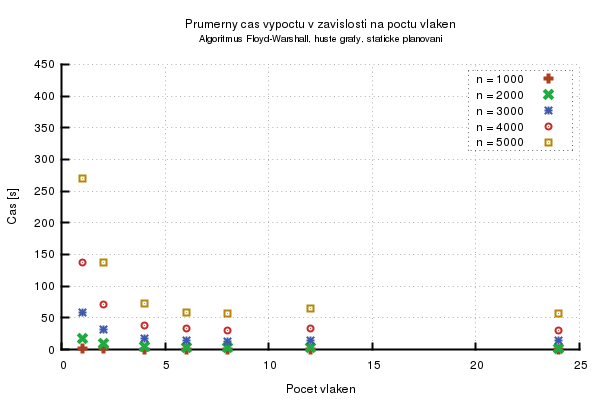
\includegraphics[width=0.45\textwidth]{../grafy/02_openMP/02-01-Floyd_cas_v3}
    \caption{Závislost průměrného času výpočtu v~závislosti na počtu vláken za použití statického plánování po optimalizaci \ref{l:opt2}.}
    \label{f:mer:cas:opt2}
\end{figure}

% Zrychleni
\begin{figure}
    \centering
    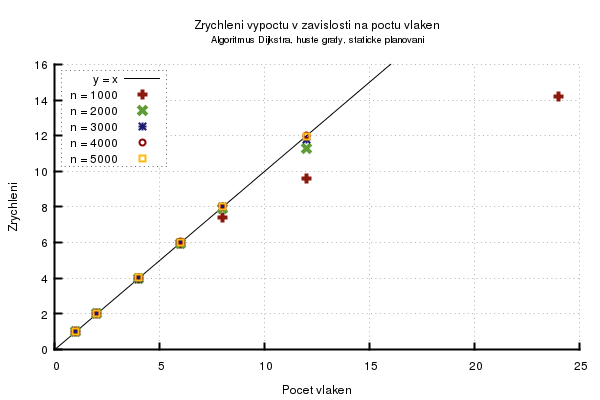
\includegraphics[width=0.45\textwidth]{../grafy/02_openMP/02-02-Dijkstra_zrychleni_v3}
    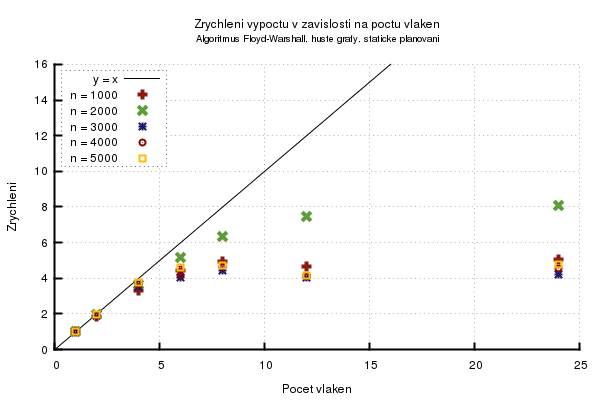
\includegraphics[width=0.45\textwidth]{../grafy/02_openMP/02-02-Floyd_zrychleni_v3}
    \caption{Závislost zrychlení paralelního algoritmu oproti sekvenčnímu v~závislosti na počtu vláken za použití statického plánovánípo optimalizaci \ref{l:opt2}.}
    \label{f:mer:zry:opt2}
\end{figure}

% Efektivita
\begin{figure}
    \centering
    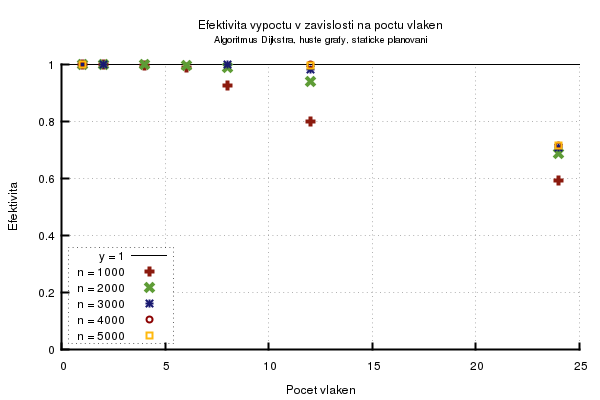
\includegraphics[width=0.45\textwidth]{../grafy/02_openMP/02-03-Dijkstra_efektivita_v3}
    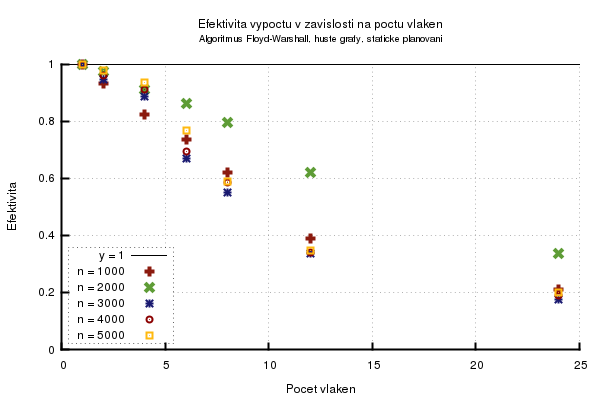
\includegraphics[width=0.45\textwidth]{../grafy/02_openMP/02-03-Floyd_efektivita_v3}
    \caption{Závislost efektivity algoritmu v~závislosti na počtu vláken za použití statického plánování po optimalizaci \ref{l:opt2}.}
    \label{f:mer:efe:opt2}
\end{figure}

\subsubsection{Zhodnocení}
Efektivita Dijkstrova algoritmu s~přidáváním vláken pomalu klesá a~například pro 24 vláken dosahuje hodnoty 0.5. Naproti tomu u~Floyd-Warshallova algoritmu klesá efektivita mnohem rychleji a~na hodnotě 0.5 se nachází už pro 6 vláken. 

Výrazně lépe ve prospěch Dijkstrova paralelního algoritmu vycházejí i~ostatní ukazatele -- zrychlení a~čas výpočtu.

Výsledky Floyd-Warshallova algoritmu mohou být způsobeny opakovaným vytvářením a~rušením vláken. V~každém vnějším cyklu se vytvoří daný počet vláken, zpracuje jeden uzel a~všechna tato vytvořená vlákna se opět ukončí. Tedy za běhu algoritmu se vytváří a~ruší \textit{pocet\_uzlu $\times$ vlaken}, kde parametr \textit{vlaken} je počet najednou vytvářených paralelních vláken.



%-------------------------------
%---		CUDA			 ---
%-------------------------------
\section{Paralelní algoritmy pomocí technologie CUDA}
\subsection{Dijkstrův algoritmus}
Paralelizace Dijkstrova algoritmu spočívá, stejně jako u technologie openMP \ref{l:omp:dij}, v~paralelizaci cyklu, který prochází jednotlivé uzly a~pro ně řeší problém hledání nejkratší cesty v~grafu z~jednoho počátečního uzlu. Každé vlákno na grafické kartě (GPU) \cite{w:gpu} zpracovává jednu instanci s jedním uzlem jako počátečním a~z~něj hledá nejkratší cesty do všech ostatních uzlů. Na grafické kartě se tedy spouští v součtu \textit{N} vláken.

\paragraph{Počet vláken}
Pomocí přepínače \textit{-w} je možné specifikovat počet spouštěných warpů. Algoritmus si poté sám vypočte, jaký počet bloků a vláken je potřeba spustit pro daný počet uzlů \textit{N}.

\subsubsection{Paměť}
Alokace paměti v programu, který počítá na grafické kartě je rozdílná od klasické alokace v RAM, kterou používá procesor. Pro alokaci paměti na grafické kartě je nutné využívat specializované funkce pro systém Cuda. Pro alokaci pole na grafické kartě je nutné nejprve alokovat pole na příslušnou velikost a poté ještě nakopírovat ukazatel na toto pole do paměti grafické karty. Pro dvojrozměrné pole, které v algoritmu využíváme, je nutné přidat ještě další krok kopírování \textit{N} ukazatelů a pro každý z nich teprve alokovat příslušné pole.

\paragraph{Paměťové struktury na CPU}
V algoritmu je na CPU alokována \textit{matice vzdáleností}, která je použita pro sběr výsledků, kam po skončení algoritmu vlákna z GPU kopírují své výsledky.

\paragraph{Paměťové struktury na GPU}
Na GPU je alokována a inicializována jedna instance grafu, která je kopií grafu, vytvořeného na CPU. Graf je přístupný všem vláknům a slouží pouze ke čtení, proto stačí pouze jedna instance. Dále je na GPU alokován celý objekt třídy \textit{cDijkstra}, který obsahuje číslo výchozího uzlu, které je pro každé vlákno jiné, počet již uzavřených uzlů, celkový počet uzlů, ukazatel na společný graf a dvě jednorozměrná pole. První je pole \textit{vzdáleností} k ostatním uzlům, které je inicializováno na \textit{nekonečno}. Druhé pole \textit{uzavřený} definuje již uzavřené uzly, ke kterým již byla nalezena nejkratší možná cesta.

\subsubsection{Výpočet}
Samotný výpočet již zajišťuje samotná třída \textit{cDijkstra}, respektive její metoda \textit{devSpustVypocet()}, která je spuštěna v každém vlákně. Protože vlákno již má všechny potřebné paměťové struktury, může počítat nejkratší cesty v grafu z daného výchozího uzlu, aniž by bylo nutné synchronizovat se s ostatními vlákny.

\paragraph{Kopírování a výpis výsledků}
Po skončení výpočtu na všech vláknech na GPU následuje kopírování výsledků zpět do paměti RAM tak, aby data byla přístupná z CPU. CPU pak pouze vypíše připravenou matici nejkratších vzdáleností v grafu.






\subsection{Floyd-Warshallův algoritmus}
V~rámci této semestrální práce byly implementovány dvě verze paralelního zpracování Floyd-Warshallova algoritmu. 
První verze je základní algoritmus, kde je pro každý výpočet relaxace každé hrany\footnote{Relaxace hrany $i,j$ přes $k$ je operace, 
kde se do matice délky cest uloží menší ze dvou vzdáleností -- buď původní cesta z~$i$ do $j$ nebo cesta
přes $k$, tedy součet vzdáleností z~$i$ do $k$ a~z~$k$ do $j$.} voláno jedno vlákno. Dále bylo implementováno 
optimálnější paralelní Floyd-Warshallova algoritmu -- zpracování po dlaždicích, včetně efektivního použití sdílené paměti.
Měření bylo provedeno u~obou verzí a~je shrnuto v sekci \ref{l:cuda:mereni}.

\subsubsection{Základní paralelní algoritmus}
Základní naivní paralelní řešení Floyd-Warshallova algoritmu spočívá v~$N$-krát paralelním spuštění $N^2$ vláken. 
Každé vlákno vždy dostane jednu dvojici indexů $i$ a~$j$ a~má za úkol relaxovat tuto hranu $i,j$. Pro zadaný počet vláken
v~bloku roste počet bloků \emph{kvadraticky} s~počtem uzlů $N$, nicméně toto řešení strádá na propustnosti sběrnice
ke globální paměti. V každém kroku algoritmu $k$ se snaží $N^2$ vláken přistoupit ke třem -- v~drtivé většině případů -- 
různým prvkům matice. I kdyby byly všechny přístupy do paměti \emph{združené}, sběrnice je velmi úzké hrdlo pro tuto verzi
algoritmu.

% todo vysledek z profilace?

Pro konkrétní implementaci v~této práci byla zvolena velikost bloku jako volitelný parametr programu. Tato velikost bloku se zadává
jako celočíselný počet warpů ($w$), aby nedocházelo ke zbytečnému snižování efektivity výpočtu\footnote{Řadič grafické karty 
s~technologií CUDA vždy spouští celočíselný počet warpů (1 warp odpovídá 32 vláken), přičemž nežádoucí vlákna jsou deaktivována.
V~případě, že je třeba spustit jiný počet vláken, je tak efektivita výkonu grafického akcelerátoru snižována.}.
% todo možná zmínit už u Dijkstry a zde se na to odkázat.
Počet bloků se pak dopočítá tak, aby bylo celkově spuštěno minimálně $N^2$ vláken. Tedy počet bloků $B = \lceil \frac{N^2}{w*32} \rceil$.

\subsubsection{Optimalizace pro paralelní výpočet}
Optimalizace pro paralelní výpočet na akcelerátoru CUDA byla zpracována dle \ref{floyd-cuda}. Prvním krokem bylo rozdělit výpočet 
celé matice najednou do výpočtu po (pevně velkých) dlaždicích. Touto optimalizací se zvyšuje prostorová lokalita dat a zvyšuje
se tak \emph{cache-hit} pravděpodobnost. V tomto parlalním zpracování se každý blok vláken stará pouze o jednu dlaždici
a je tak možné využít sdílenou paměť, kterou mohou společně využít vlákna v~jednom bloku.

\paragraph{Dlaždicové zpracování}
V tomto přístupu výpočtu je daná matice délek cest rozdělena do pevně velkých dlaždic. Iterování~v průbehu algoritmu je pak
upraveno podle klasické metody \emph{proložení cyklů} (\emph{loop tiling}) -- tedy kde $k1$ iteruje přes počet dlaždic 
a~$k2$ přes velikost dlaždice. Výpočet každé iterace $k1$ je pak dále rozdělen do
3 sekcí -- výpočet pro \emph{nezávislé dlaždice}, pro \emph{jedno-závislé dlaždice} a \emph{dvou-závislé dlaždice}.
\begin{enumerate}
    \item \textbf{Výpočet pro nezávislé dlaždice} \label{cuda:dlazdice:nezavisle} \\
        Jedná se o výpočet dlaždice ležící na hlavní diagonále matice. Pro každé $k1$ i~$k2$ je mezilehlý uzel $k$ uvnitř této
        dlaždice a výpočet relaxace všech hran je tedy velmi lokalizovaný. Všechny přístupy do paměti jsou pouze v rámci této 
        jedné dlaždice.

    \item \textbf{Výpočet pro jedno-závislé dlaždice} \label{cuda:dlazdice:jednozavisle} \\ 
        Tyto dlaždice vždy leží ve stejném řádku (resp. sloupci)\footnote{Dále nazýváno jako \emph{hlavní řádek} (resp.
        \emph{sloupec}) dlaždic.} jako dlaždice z~bodu~1. Pro tyto dlaždice platí, že hrana do 
        mezilehlého uzlu $k$ leží v~matici z~bodu 1. a hrana z~uzlu $k$ v~jedno-závislé dlaždici samotné (resp. pro sloupce je to 
        přesně naopak). Výpočet je tak velmi lokalizovaný, neboť každý blok čte pouze z~dlaždice samotné a z~matice z~bodu 1.

    \item \textbf{Výpočet pro dvou-závislé dlaždice} \label{cuda:dlazdice:dvouzavisle} \\
        Jedná se o výpočet pro všechny ostatní dlaždice nezpracované v~předešlých krocích. Pro všechny tyto dlaždice platí, že 
        hodnota hran do i~z~mezilehlého uzlu $k$ leží v dlaždicích vypočítaných v~kroku 2.. Přesněji potřebné hodnoty pro výpočet
        jedné \emph{dvou-závislé} dlaždice leží v~dlaždici samotné a právě ve dvou dlaždicích spočítaných v kroku 2. První, 
        z~\emph{hlavního sloupce} je ve stejném řádku a~druhá, z~\emph{hlavního řádku}, je ve stejném sloupci. Opět je tak 
        výpočet velmi lokalizovaný -- pro výpočet jedné dlaždice se opakuje přístup ke stejným hodnotám na malém prostoru v paměti.

\end{enumerate}

\paragraph{Použití sdílené paměti a registrů}\label{cuda:sdilena}
V~případě, že se jeden blok vždy stará právě o~jednu dlaždici, je možné iterování přes $k2$ řešit uvnitř kernelu. 
Pak v~případě výpočtu \emph{dvou-závislých} dlaždic každý blok pracuje s~daty právě ze tří dlaždic:
\begin{itemize}
    \item dlaždice samotné, kde se zapisují nově nalezené hodnoty
    \item jedna dlaždice z~\emph{hlavního sloupce} a jedna dlaždice z~\emph{hlavního řádku}, ze kterých se čtou hodnoty
        pro mezilehlý uzel $k$
\end{itemize}

Pro jednu konkrétní hranu $i,j$ a~velikost dlaždice $s$ se uvnitř kernelu provádí $s$ čtení a $s$ zápisů prvku $i,j$ matice ($M_{i,j}$).
Dále se čtou opakovaně hodnoty z~dlaždice z~\emph{hlavního sloupce} resp. \emph{řádku} -- pro všech $s$ hran z~jednoho řádku se čte
daná hodnota pro index $k2$ z~dlaždice z~\emph{hlavního sloupce} a stejně tak pro všech $s$ hran z~jednoho sloupce se čte daná hodnota
pro index $k2$ z~dlaždice z~\emph{hlavního řádku}. V~průběhu iterování $k2$ se tak čte každá hodnota z~dlaždice z~\emph{hlavního sloupce} 
i~\emph{řádku} a $s$-krát.

Jelikož o výpočet pro jednu dlaždici se stará právě jeden blok vláken, je možné využít sdílenou paměť a~uštřit tak čas kvůli opakovanému 
čtení stejný položek z matice. Na začátku kernelu se načtou 2 dlaždice z~\emph{hlavního řádku} a~sloupce do sdílené paměti a~v~průběhu 
výpočtu se pak používají data z~této sdílené paměti. Jelikož se tato data používají jen pro čtení, není třeba je zpět zapisovat do 
hlavní paměti.

Pro optimalizaci algoritmu byly implementovány různé kernely pro pevný počet warpů. Díky tomu je možné dlaždici samotnou -- která je 
kernelem zpracovávána -- uložit do registrů. Každé vlákno si na začátku kernelu uloží do vlastních registrů hodnoty $M_{i,j}$, které
má na starost a~výpočet provádí v~registrech. Před ukončením kernelu každé vlákno uloží výsledná data z~registrů uloží zpět do hlavní 
paměti.

Kvůli úpravě algoritmu pro použití registrů jsou implementovány kernely pouze pro počet warpů rovný mocninám dvou.

\paragraph{Fázové zpracování}
Jak již bylo řečeno v~\ref{cuda:sdilena}, tak pro výpočet \emph{dvou-závislých} dlaždic se opakovaně čte jedna hodnota z~dlaždic 
z~\emph{hlavního řádku} resp. \emph{sloupce}. Koknrétně v~iteraci danou hodnotou $k$ se čte sloupec matice $M_{i,k}$ a~řádek matice
$M_{k,j}$. Tedy při omezení na dlaždicové zpracování se pro výpočet celé dlaždice v~iteraci $k$ čte pouze jeden sloupec z~dlaždice
z~\emph{hlavního sloupce} a~jeden řádek z~dlaždice z~\emph{hlavního řádku}. V~průběhu iterování přes $k2$ není tedy třeba si udržovat 
ve sdílené paměti celé dlaždice z~\emph{hlavního řádku} resp. sloupce.

Tato skutečnost se dá využít pro fázové načítání dat do sdílené paměti, čímž se radikálně ušetří požadavky na velikost sdílené paměti
pro jeden blok. Místo toho, aby se data z~dlaždic načetla do sdílené paměti na začáctku kernelu, se načítá potřebný sloupec (resp. řádek)
do sdílené paměti v~každé iteraci přes $k2$. Pro správný průběh výpočtu a načítání dat v průběhu iterování je potřeba vlákna synchronizovat
bariériou v~každé iteraci.


\subsubsection{Profilace}


\subsubsection{Efektivnost využití akcelerátor}
Následující výpočet efektivnosti využití \emph{gpu} byl spočítán pro graf o~5000 uzlech a 4 warpy (128 vláken v bloku).
Měření bylo prováděno na grafické kartě \emph{GeForce GTX 780 Ti} (\emph{Cuda CC 3.0}), pro kterou platí hardwarové omezení 
dle tabulky \ref{tab:cuda:hw}.

\begin{table}[h!]
    \centering
    \begin{tabular}{lll}
        \hline
        Vlastnost                & Označení & Hodnota \\
        \hline
        Počet SM                 & $#SM$    & 15      \\
        \hline
        \emph{Vlastnosti na 1 SM:} &        &
        \hline
        Počet bloků              & $BlMax$  & 16      \\
        Počet registrů           & $RegMax$ & 64 k    \\
        Velikost sdílené paměti  & $ShMax$  & 48 kB   \\
        \hline
    \end{tabular}
    \caption{Hardwareové vlastnosti karty GeForce GTX 780 Ti \cite{pap:prednasky}}
    \label{tab:cuda:hw}
\end{table}


Spouštený počet bloků ($#SB$)odpovídá počtu dlaždic matice vzdáleností. Pro $5000$ uzlů a velikost dlaždice $32$ je to 
$\lceil \frac{5000}{32} \rceil ^ 2 = 24649$. Počet vláken $#V$ je tedy 128 (4 warpy).

V~každém bloku se vždy spouští přesně 4 warpy ($ #Wb $), ale celkově se matice $5000 \times 5000$ musi zarovnat na celočíselný násobek
dlaždic, tedy na $5024$ a je tak třeba provádět výpočet i~pro neexistující prvky. Celkový počet prvků navíc je tedy $ 5024^2 $, kde 
užitečných počet prvků je $ 5000^2 $. Efektivita pro počet užitečných vláken je tedy
$$ E_1 = \frac{5000^2}{5024^2} = 99.05 \% $$


Dle \ref{cuda:fw:profilace} zabírá každé vlákno \emph{25} registrů ($#reg$) a~každý blok \emph{256~B} sdílené paměti $#ShM$. Pro rezidentní počet 
bloků na jednom SM ($#B$)  platí následující nerovnice:
$$             #B \leq BlMax   \Rightarrow  #B \leq 16    $$
$$ #B . #V . #reg \leq RegMax  \Rightarrow  #B \leq 20.48 $$
$$      #B . #ShM \leq ShMax   \Rightarrow  #B \leq 192   $$

Z nerovnic tedy vyplývá, že počet rezidentních bloků na jednom \emph{SM} je 16. Celkový počet rezidentních bloků $ #RB = #B * #SM = 240 $.

Počet iterací\footnote{V případě, že výpočet všech bloků trvá stejně dlouho. To v~tomto případě platí, protože je algoritmus datově necitlivý.}
je $ #it = \lceil \frac{#SB}{#RB} \rceil = 103 $. Efektivita využití \emph{SM} je tedy 

$$ E_2 = \frac{#SB}{#it . #RB } = 99.7 \% $$

% TODO latence operaci
Počet rezidentních warpů na jednom \emph{SM} je  $ #W = #B . #Wb = 64 $. To je více než nejdelší latence instrukcí a proto efektivita prokládání 
warpů je 

$$ E_3 = 100 \% $$


Celková efektivita je 
$$ E = E_1 . E_2 . E_3  = 98.8 \% $$

\subsection{Měření}\label{l:cuda:mereni}
\subsubsection{Analýza}
\subsubsection{Zhodnocení}


\section{Závěr}




\clearpage
\bibliographystyle{czechiso} % nutny soubor czechiso.bst
\bibliography{citace}

\end{document}


